%!TEX root=./LIVRO.tex
\chapter{Representações numéricas}

\section{Habilidades do SAEB}

\begin{itemize}

\item
  Escrever números racionais (representação
  fracionária ou decimal finita) em sua representação por algarismos ou em
  língua materna ou associar o registro numérico ao registro em língua
  materna.
\item
  Compor ou decompor números racionais positivos (representação decimal
  finita) na forma aditiva, ou em suas ordens, ou em adições e
  multiplicações.
\item
  Identificar números racionais ou irracionais.
\item
  Comparar ou ordenar números reais, com ou sem suporte da reta
  numérica, ou aproximar número reais para múltiplos de potência de 10
  mais próxima.
\item
  Converter uma representação de um número racional positivo para outra
  representação.
\item
  Identificar um número natural como primo, composto, ``múltiplo/fator
  de'' ou ``divisor de'' ou identificar a decomposição de um número
  natural em fatores primos ou relacionar as propriedades aritméticas
  (primo, composto, ``múltiplo/fator de'' ou ``divisor de'') de um
  número natural à sua decomposição em fatores primos.
\end{itemize}



\conteudo{As representações numéricas são sistemas utilizados para expressar quantidades e valores numéricos 
de forma organizada e compreensível. Essas representações desempenham um papel fundamental em diversas áreas.
Existem diferentes tipos de representação numérica; cada uma é adequada para uma finalidade específica. 
Algumas das representações mais comuns são:

A representação decimal é baseada no sistema decimal, que utiliza dez dígitos ($0$ a $9$). Cada posição em um número decimal tem um valor associado a potências de dez. Por exemplo, o número $358$ 
é representado como a soma de $3 x 10^2 + 5 x 10^1 + 8 x 10^0$.

A representação binária é baseada no sistema binário, que utiliza apenas dois 
dígitos ($0$ e $1$). Cada posição em um número binário tem um valor associado a potências de dois. Por exemplo, o 
número binário 101 é representado como a soma de $1 x 2^2 + 0 x 2^1 + 1 x 2^0$, que é igual a 5 em decimal.

A representação hexadecimal é baseada no sistema hexadecimal, que utiliza 
dezesseis dígitos ($0$ a $9$ e $A$ a $F$). A base 16 é utilizada para representar números grandes e facilitar a 
conversão entre binário e decimal. Por exemplo, o número hexadecimal 2A é representado como a soma de 
$2 x 16^1 + A x 16^0$, onde $A$ tem o valor de $10$ em decimal. Portanto, $2A$ em hexadecimal é igual a $42$ em decimal.

A representação de ponto flutuante é usada para representar números 
reais, que podem ter uma parte inteira e uma parte fracionária. Esse sistema é comumente usado em computação 
para representar números com uma quantidade limitada de dígitos. É baseado em notação científica, em que um 
número é expresso como uma mantissa multiplicada por uma potência de base fixa.

As representações numéricas são essenciais para realizar operações matemáticas, armazenar e transmitir 
dados, e implementar algoritmos em diversas áreas. O conhecimento e o entendimento das diferentes 
representações numéricas são fundamentais para evitar erros de arredondamento, compreender as limitações dos 
sistemas de numeração e garantir a precisão e confiabilidade dos cálculos numéricos.}

\section{Atividades}

\num{1} Calculando-se $(\sqrt{27})$, obtém-se $5,196152423$..., número que tem
representação decimal infinita, mas não é dízima periódica.

Conclui-se então que $(\sqrt{27})$ é um número:

\reduline{ Irracional.}


\num{2} O número romano XLV corresponde, em algarismos arábicos, a

\reduline{$45$}

\num{3} Observe os números a seguir:

\begin{figure}[H]
\centering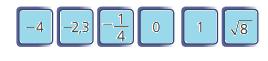
\includegraphics[width=2.79167in,height=0.63542in]{./imgSAEB_8_MAT/media/image1.png}
\end{figure}

Quais deles pertencem ao conjunto:


\begin{escolha}
\item N \rosa{-- $0; 1$}
\item Z \rosa{-- $-4, 0, 1$}
\item Z, mas não pertencem a N? \rosa{$-4$}
\item Q, mas não pertencem a Z? \rosa{$-2,3$ e  $(-\frac{1}{4})$}
\end{escolha}
\num{4} Observe os números abaixo:

$$6; (\sqrt{6}); 6,6; -6$$

\begin{comment}

Identifique quais deles são:
\begin{escolha}
\item reais e naturais.\rosa{ -- 6}
\item reais e inteiros.\rosa{ -- 6 ; -6}
\item reais e racionais.\rosa{ -- 6; -6; 6,6}
\item reais e irracionais.\rosa{-- (\sqrt{6})}
\end{escolha}


\num{5} Complete os espaços abaixo com pertence ou não pertence:


\begin{multicols}{3}
\def\labelenumi{\alph{enumi})}
\begin{enumerate}
\item 100 
\item 100 
\item 100 
\item (\sqrt{9}) 
\item - (\sqrt{9}) 
\item (\sqrt{- 9}) 
\item 2,6 
\end{enumerate}


\begin{enumerate}
R*
R\textsubscript{+}
R\textsubscript{-}
R
R
R
R\textsubscript{+}
\end{enumerate}

\begin{enumerate}
++R:
\rosa{-- Pertence}
\rosa{-- Pertence}
\rosa{-- Não Pertence}
\rosa{-- Pertence}
\rosa{-- Pertence}
\rosa{-- Não Pertence}
\rosa{-- Pertence\end{enumerate}
\end{multicols}

\num{6} A representação decimal de um número pode ser: finita, infinita e
periódica ou, ainda, infinita e não periódica. Escreva qual é o caso de
cada um dos números a seguir

\begin{escolha}
\item(\frac{15}{6}) \rosa{-- Finita}
\item(\frac{1}{3}) \rosa{-- Infinita e periódica}
\item (\sqrt{3}) \rosa{-- Infinita e não periódica}
\item (\sqrt{2}) \rosa{-- Infinita e não periódica}
\end{escolha}

\num{7} O número (\pi) é classificado como:

\reduline{ uma dízima não periódica.}

\num{8} O números $121$ é considerado um quadrado perfeito? Por quê?

Sim, pois $121 = 11 x 11$.

\num{9} O produto ou o quociente de dois números irracionais pode ser um
número racional?

\reduline{ Sim, como exemplos podem ser citados }
\reduline{ $(\sqrt{2}) x (\sqrt{2}) = ((\sqrt{2})) ^2 = 2$ e também $(\frac{\sqrt{2}}{\sqrt{2}}) = 1}$

\num{10} Qual é o menor número natural que devemos multiplicar pelo número
125 para que o produto seja um número quadrado perfeito?

\reduline{ $5$, pois $5 x 125 = 625$ e $(\sqrt{625}) = 25$.}

\end{comment}
